% !TEX TS-program = pdflatex
\documentclass[12pt]{report}

% Package the packages
\usepackage[T1]{fontenc}
\usepackage[utf8]{inputenc}
\usepackage{lmodern}
\usepackage[a4paper, margin=1in]{geometry}
\usepackage{enumitem}
\usepackage[colorlinks=true, linkcolor=black, citecolor=black, urlcolor=blue]{hyperref}
\usepackage[nottoc,numbib]{tocbibind}
\usepackage[round]{natbib}
\usepackage{pdfpages}
\usepackage{fancyvrb}
\usepackage[parfill]{parskip}
\usepackage{titlesec}
% -

% Configuration
% Change font to Palatino
\renewcommand{\rmdefault}{ppl}
% Change the list item spacing
\setlist{noitemsep}
% Set the bibliography style
\bibliographystyle{usw}
% Set up a terminal command block
\definecolor{light-gray}{gray}{0.95}
\newcommand{\term}[1]{\colorbox{light-gray}{\texttt{#1}}}
% Set up better chapter titling
\titleformat{\chapter}{\normalfont\huge\bfseries}{\thechapter.}{10pt}{}
\titlespacing{\chapter}{0pt}{0pt}{12pt}
\titleformat{\section}{\normalfont\Large\bfseries}{\thesection}{10pt}{}
\titleformat{\subsection}{\normalfont\large\bfseries}{\thesubsection}{10pt}{}
% -

% Definitions
\title{IY1D402\thanks{University of South Wales, National Cyber Security Academy}\\{\textit{\small Cyber Security Tools And Practices}}\\Assessment 1 Remote Exploitation Report}
\author{David Sanders\\{\LARGE 17135397}}
\date{\today}
% -

% Document
\begin{document}

% Cover page setup
\maketitle
\pagebreak
% 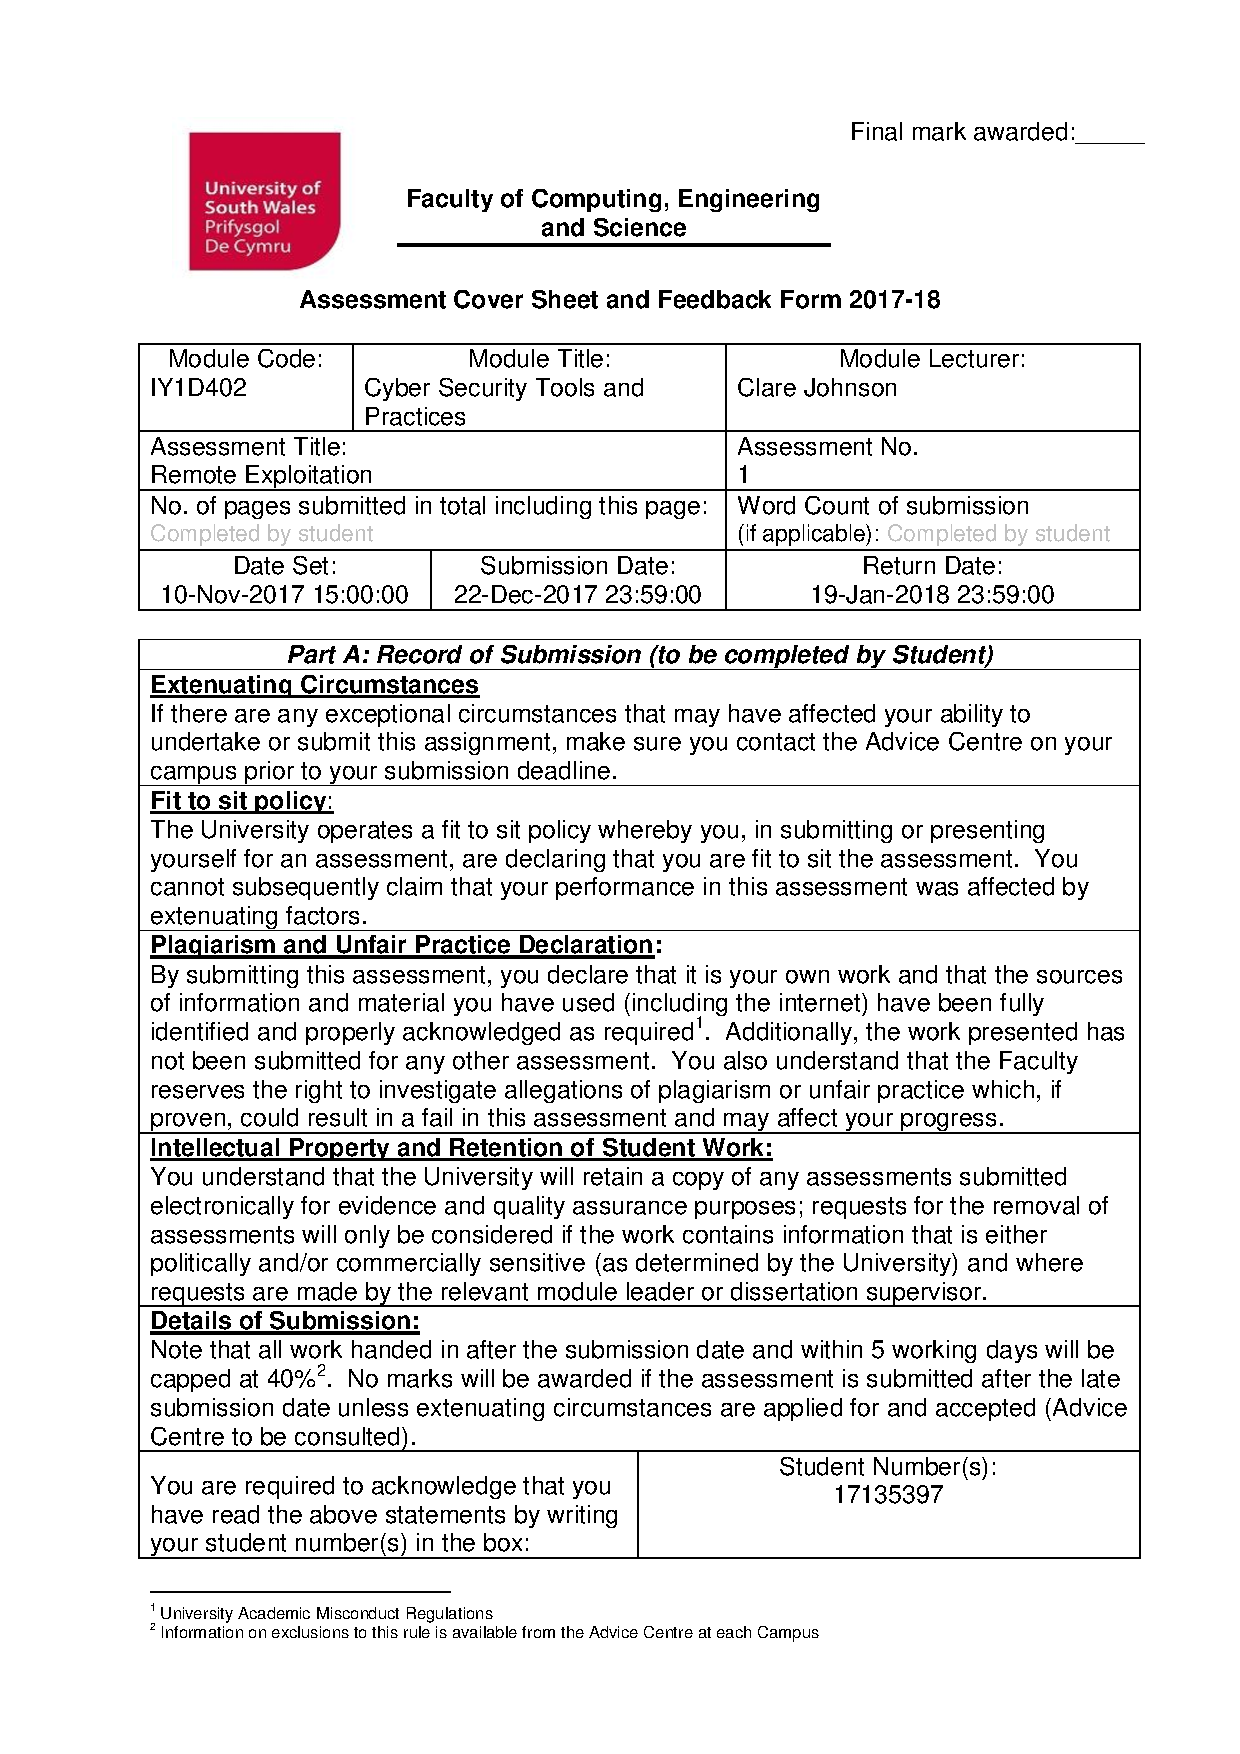
\includepdf[pages={1}]{assignmentbrief/IY1D402_CW1M_Cover_PRO_PROJECT1.pdf}
\tableofcontents
% -

% Introduction
\pagebreak
\chapter{Introduction}
For the first formal assessment of our IY1D402 \textit{(Cyber Security Tools and Practices)} we have been given a real-world scenario. We have been asked to, individually, conduct an investigation before writing a report that details the methodology that we followed during our investigation, presents our findings, discusses the capabilities of the tools we used, describes alternative methods that could have been used, and explains the nature of \textit{'insider threat'}. The target audience is a Senior Management Team and so, although it is a technical, this report will attempt to present technical aspects with enough explanation to make them understandable by those who are not technical specialists.

\section{Scenario}
I am the Senior Technical Officer at eCorp and have been asked by the Senior Management Team to investigate an employee -- Phillip Price -- who is suspected of exfiltrating Intellectual Property (IP) from the company.

To verify this suspicion, I have been asked to monitor Price's activities on the company's IT system, and have been given permission to use any appropriate methods in the course of this investigation. It has also been requested that I take suitable steps to conceal this monitoring from Price.

Upon completion of the investigation, I have been asked to write a report for the Senior Management Team that details exactly the steps that I took and explains my findings. I should also discuss the capabilities of the tools that I used and explain whether any alternative methods could have been used at various stages of the investigation.

Finally, to complete the report, I should explain the nature of \textit{'insider threat'} and its implications to an organisation while giving examples of where such threats have occurred in the past, discussing how the tools that I used impact on the organisation's security, and suggesting methods for improving our security in the future.

To aid in my investigation, I have been provided with a list of commonly used passwords that might help me to gain access to Price's machine.
% -


% Glossary
\pagebreak
\chapter{Glossary}
todo: Maybe add a glossary - one would probably included in this sort of technical report (that is, one with a not necessarily technical audience)
% -


% Preliminary Report
\pagebreak
\chapter{Preliminary Report}
During the investigation, I gathered a lot of information regarding Price's machine and account. I will summarise the most important points in a table below and detail fully the methodology by which I acquired this information in the next chapter of the report.

\begin{table}[h!]
  \centering
  \begin{tabular}{|r l|}
    % \hline
    % \multicolumn{2}{||l||}{Information} \\
    % \hline\hline
    \hline
    IP address: & 192.168.254.132 \\
    \hline
    Operating system: & Ubuntu \\
    \hline
    % Open Ports\footnotemark : & [details the ports] \\
    Open ports: & 80 \textit{[http]}, 442 \textit{[ssh; OpenSSH 7.5p1 Ubuntu 10]} \\
    \hline
    Closed ports: & 443 \textit{[https]} \\
    \hline
    Price's groups: & [groups here] \\
    \hline
  \end{tabular}
  \caption{Information on Price's machine and account}
  \label{table:pricemachineinfo}
\end{table}
% \footnotetext{Common and in-range 1-1000}

The IP address was found by scanning the network with arp-scan, and the operating system and ports were found using Nmap.
% -


% Investigate Methodology
\pagebreak
\chapter{Investigative Methodology}
In this section of the report, I will describe in detail the steps that I took to find, gain access to, and monitor Price's machine during the investigation. In order to keep this section of the report as concise as possible, I have included evidential deliverables (screenshots and code) of some of the steps in the process in the appendices.


\section*{Setting up the Virtual Machines}
Due to the way in which the hypothetical scenario was presented, I had to set up two virtual machines in VMWare Workstation in order to conduct the analysis of the Price's machine. In reality, Price's machine would most likely be a physical computer connected to the eCorp network.

Firstly, I set up a new VM \textit{('eCorp Target?')} using the VMDK (Virtual Machine Disk) image of Price's machine that we had been provided. I configured the network adaptor in this machine to connect to a host-only network, which was provided by the VMWare software.

Secondly, I configured my existing attack VM \textit{('elementaryos-vm?')} to have two network adaptors - the existing NAT adaptor, which allows it to connect to the Internet, and the host-only network adaptor.

After completing this steps, I \textit{'powered on'} both of the virtual machines.


\section{Searching the network}
The first stage of investigation is to find the IP address of Price's machine on the network -- in the real world, this IP would likely be provided to us by the network administrator. However, even though it would be harder to do in a network with more than two machines, I will describe how I used \texttt{ifconfig} and \texttt{arp-scan} to find the IP address.

\subsection{Using \texttt{ifconfig} to find the host-only network interface name}
In order to be able to use \texttt{arp-scan} in the second part of this stage, I needed to know the interface name of the host-only network on the attack VM. To find the interface name I used the \term{ifconfig} command.

As we know that the NAT adaptor interface is called \textit{ens33}, the relevant output of this command is:
\begin{Verbatim}[frame=leftline]
ens34     Link encap:Ethernet  HWaddr 00:0c:29:72:88:f2
          inet addr:192.168.254.135  Bcast:192.168.254.255  Mask:255.255.255.0
          inet6 addr: fe80::490:c374:f983:b700/64 Scope:Link
          UP BROADCAST RUNNING MULTICAST  MTU:1500  Metric:1
          RX packets:52792 errors:0 dropped:0 overruns:0 frame:0
          TX packets:56528 errors:0 dropped:0 overruns:0 carrier:0
          collisions:0 txqueuelen:1000
          RX bytes:9729912 (9.7 MB)  TX bytes:10084091 (10.0 MB)
\end{Verbatim}

From this, we can discern that the host-only interface name is \textit{ens34}.

\subsection{Using \texttt{arp-scan} to find the IP address of Price's machine}
In order to discover the IP addresses of machines in the network I used the command:\\
\term{sudo arp-scan -lI ens34}

The output of this command was:
\begin{Verbatim}[frame=leftline, fontsize=\small]
Interface: ens34, datalink type: EN10MB (Ethernet)
Starting arp-scan 1.8.1 with 256 hosts (http://www.nta-monitor.com/tools/arp-scan/)
192.168.254.1	00:50:56:c0:00:01	VMware, Inc.
192.168.254.132	00:0c:29:e2:a5:34	VMware, Inc.
192.168.254.254	00:50:56:ed:f1:b4	VMware, Inc.

3 packets received by filter, 0 packets dropped by kernel
Ending arp-scan 1.8.1: 256 hosts scanned in 1.342 seconds (190.76 hosts/sec). 3 responded
\end{Verbatim}

As my attack machine IP is not shown and 192.168.254.1/254 are \textit{services} operated by VMWare to support the operation of the host-only network, I can see that \textbf{192.168.254.132} must be the IP address of the Price's machine.

\subsubsection{Capabilities}
todo: detail the capabilities - maybe move these sections into a separate chapter
\subsubsection{Alternative tools/methods}
todo: detail alternative methods


\section{Scanning Price's machine}
With the IP address of Price's machine, I used Nmap to scan the machine for open ports and find the SSH service.
\subsection{Running a basic Nmap scan}
Initially, I ran a basic Nmap scan using:\\
\term{sudo nmap 192.168.254.132}

The result of this scan was:
\begin{Verbatim}[frame=leftline]
Starting Nmap 7.01 ( https://nmap.org ) at 2017-12-06 13:31 GMT
Nmap scan report for 192.168.254.132
Host is up (0.00045s latency).
Not shown: 998 filtered ports
PORT    STATE  SERVICE
80/tcp  open   http
443/tcp closed https
MAC Address: 00:0C:29:E2:A5:34 (VMware)

Nmap done: 1 IP address (1 host up) scanned in 17.56 seconds
\end{Verbatim}

From this scan, I can see that port 80 is open and port 443 is closed. Connecting to the machine with a browser brings up a web page and so I can tell that the machine is definitely serving http requests on port 80. I did not find the SSH port in this scan and so it must have been moved from the port 22 (the default) to a different port.

\subsection{Expanding the scan to find the SSH port}
In order to try and find the SSH port without having to run a complete scan of all 65535 ports, I decided to run a scan of ports 1-1000 to see if the SSH service had been moved to a port in this range. To do this, I used the command:\\
\term{sudo nmap -p 1-1000 192.168.254.132}

The result of this command was:
\begin{Verbatim}[frame=leftline]
Starting Nmap 7.01 ( https://nmap.org ) at 2017-12-06 13:34 GMT
Nmap scan report for 192.168.254.132
Host is up (0.00045s latency).
Not shown: 997 filtered ports
PORT    STATE  SERVICE
80/tcp  open   http
442/tcp open   cvc_hostd
443/tcp closed https
MAC Address: 00:0C:29:E2:A5:34 (VMware)

Nmap done: 1 IP address (1 host up) scanned in 14.16 seconds
\end{Verbatim}

This scan revealed that there was a service running on open port 442. Although Nmap identifies this service as \textit{cvc\_hostd}, the service identification method used in basic Nmap scans only uses port number to guess the service.

\subsection{Using service detection to confirm the SSH port}
I used service detection to see if the SSH port had been moved to port 442. To do this, I used the command:\\
\term{sudo nmap -sV -p 442 192.168.254.132}

The result of this command was:
\begin{Verbatim}[frame=leftline]
Starting Nmap 7.01 ( https://nmap.org ) at 2017-12-06 13:38 GMT
Nmap scan report for 192.168.254.132
Host is up (0.00041s latency).
PORT    STATE SERVICE VERSION
442/tcp open  ssh     OpenSSH 7.5p1 Ubuntu 10 (Ubuntu Linux; protocol 2.0)
MAC Address: 00:0C:29:E2:A5:34 (VMware)
Service Info: OS: Linux; CPE: cpe:/o:linux:linux_kernel

Service detection performed.
Please report any incorrect results at https://nmap.org/submit/ .
Nmap done: 1 IP address (1 host up) scanned in 1.20 seconds
\end{Verbatim}

This command asked Nmap to attempt to do service detection against only port 442 on 192.168.254.132 and the result shows that the SSH service \textit{[version: OpenSSH 7.5p1 Ubuntu 10 (Ubuntu Linux; protocol 2.0)]} has been moved to this port.


\section{Breaking into Price's account}
todo: discuss how I used Python to break into Price's account

\section{Examining Price's account}
todo: talk about examining the /var/log/auth.log and /etc/passwd files

\section{Setting up persistent access to the machine}
todo: explain how to set up persistent access to the machine by creating a new account, making it superuser, and hiding it from Price

\section{Setting up a proxy to monitor traffic}
todo: explain how to set up squid on the attack machine

todo: explain how to get Price's machine to route web traffic through the proxy

\section{Concealing the investigation from Price}
todo: discuss steps that I took to conceal the investigation from Price, and detail some further methods that I could have taken


\pagebreak
\chapter{Insider Threat}
todo: write a report on insider threat...


\pagebreak
\chapter{Conclusion}
todo: brood and conclude


% Post-main configuration
% Increase the line spacing to 1x(=1.0), 1.5x(=1.3) or 2x(=1.6)
% \linespread{1.0}
% \selectfont


% BIBLIOGRAPHY/REFERENCES
% \pagebreak
% nocited refs
\nocite{example:referenceid:here}

% Insert references section, left aligned
\begin{flushleft}
  \bibliography{references}
\end{flushleft}


% APPENDICES
\appendix

\pagebreak
\chapter{Screenshot deliverables}

\pagebreak
\chapter{Code deliverables}


\end{document}
